% Correcting Forward Model Mismatch in Coded Aperture Snapshot Spectral
% Imaging via Two-Stage Differentiable Calibration
%
% ECCV-style conference paper

\documentclass[runningheads]{llncs}
\usepackage[T1]{fontenc}
\usepackage{graphicx}
\usepackage{amsmath,amssymb}
\usepackage{booktabs}
\usepackage{multirow}
\usepackage{xcolor}
\usepackage{hyperref}
\usepackage{cleveref}
\usepackage{subcaption}
\usepackage{array}
\usepackage{algorithm}
\usepackage{algorithmic}

% Custom column type
\newcolumntype{C}[1]{>{\centering\arraybackslash}p{#1}}

% Color definitions
\definecolor{bestcolor}{rgb}{0.0, 0.5, 0.0}
\definecolor{worstcolor}{rgb}{0.7, 0.0, 0.0}

\newcommand{\best}[1]{\textbf{#1}}
\newcommand{\worst}[1]{\textcolor{worstcolor}{#1}}
\newcommand{\gain}[1]{\textcolor{bestcolor}{+#1}}

\begin{document}

\title{Correcting Forward Model Mismatch in Coded Aperture Snapshot Spectral Imaging via Two-Stage Differentiable Calibration}
\titlerunning{Differentiable CASSI Calibration}

\author{Chengshuai Yang\thanks{\href{mailto:integrityyang@gmail.com}{integrityyang@gmail.com}}}
\authorrunning{C. Yang}
\institute{NextGen PlatformAI C Corp}

\maketitle

% ============================================================================
% ABSTRACT
% ============================================================================
\begin{abstract}
Forward model mismatch---sub-pixel mask misalignment and dispersion drift between the coded aperture and detector---is unavoidable in deployed CASSI systems, yet even moderate perturbations degrade state-of-the-art mask-guided transformers (MST) by over 16\,dB.
We present a self-supervised two-stage differentiable calibration pipeline that recovers 5-parameter mismatch from a single measurement and nominal mask alone, requiring no ground truth.
Stage~1 performs a coarse hierarchical grid search scored by GPU-accelerated GAP-TV; Stage~2 applies gradient refinement through an unrolled differentiable forward operator using a Straight-Through Estimator (STE) for integer dispersion offsets.
Evaluating five reconstruction methods across four scenarios on 10 KAIST scenes, we uncover a \emph{mask-sensitivity spectrum}: mask-guided transformers suffer catastrophic degradation ($>$15\,dB) yet recover ${\sim}48$\% of the oracle gap after calibration, while deep prior methods show inherent robustness with negligible absolute gain.
Code and results are publicly available.

\keywords{CASSI \and Operator mismatch \and Differentiable calibration \and Straight-Through Estimator \and Hyperspectral imaging}
\end{abstract}

% ============================================================================
% 1. INTRODUCTION
% ============================================================================
\section{Introduction}
\label{sec:intro}

Deep learning has transformed hyperspectral image reconstruction, with mask-guided transformers (MST)~\cite{cai2022mst,cai2022mst_pp} achieving $>$34\,dB on the KAIST benchmark~\cite{choi2017kaist}.
Yet these reconstructors depend on accurate knowledge of the forward operator---a dependency that creates a \emph{sim-to-real gap} between the idealized model used during training and the physical system at deployment~\cite{ongie2020deep}.
In coded aperture snapshot spectral imaging (CASSI)~\cite{wagadarikar2008cassi,arce2014cassi}, this gap manifests as mask-detector misalignment and dispersion drift, degrading MST-L by over 16\,dB (\Cref{fig:scenario_comparison}).

The CASSI forward model (\Cref{sec:formulation}) maps a hyperspectral cube through a coded aperture and spectral disperser to a 2D measurement.
In practice, five parameters characterize the dominant misalignment between the assumed and actual forward operator: mask translation $(\Delta x, \Delta y)$, rotation $\theta$, dispersion slope $a_1$, and axis angle $\alpha$.

\textbf{The calibration challenge.}
Correcting this mismatch is difficult because: (1)~spectral dispersion offsets $d_k$ are integers, making the forward operator non-differentiable; (2)~mask affine and dispersion parameters interact through the measurement model; and (3)~in deployment, neither the true parameters nor the ground truth scene are available---calibration must be self-supervised from the measurement alone.

\textbf{Contributions.} We address these challenges with:
\begin{enumerate}
    \item A \textbf{differentiable CASSI forward model} using a Straight-Through Estimator (STE)~\cite{bengio2013ste} for integer dispersion offsets, enabling end-to-end gradient-based calibration (\Cref{sec:method}).
    \item A \textbf{two-stage self-supervised calibration pipeline} (\Cref{alg:calibration}): coarse grid search followed by gradient refinement, recovering 5-parameter mismatch from a single measurement without ground truth.
    \item A \textbf{mask-sensitivity spectrum} characterizing how five reconstructors respond to mismatch and calibration: mask-guided methods (MST-S/L) suffer ${>}$15\,dB degradation but recover $\rho {\approx}\,48$\% of the oracle gap; deep prior methods show inherent robustness; iterative methods show intermediate sensitivity (\Cref{sec:experiments}).
    \item A \textbf{four-scenario evaluation framework} (Ideal, Assumed, Corrected, Oracle) with complete open-source benchmark on 10 KAIST scenes across five methods.
\end{enumerate}

% ============================================================================
% 2. RELATED WORK
% ============================================================================
\section{Related Work}
\label{sec:related}

\textbf{CASSI reconstruction.}
Classical approaches including GAP-TV~\cite{yuan2016gap,meng2020gap} use alternating projection with total variation regularization.
Plug-and-play methods replace the hand-crafted prior with learned denoisers~\cite{yuan2020pnpcassi,zheng2021deep}, combining ADMM/GAP optimization with deep spectral denoisers.
End-to-end deep networks have advanced quality through dual-domain unfolding (HDNet~\cite{hu2022hdnet}), mask-guided attention (MST~\cite{cai2022mst,cai2022mst_pp}), sparse transformers (CST~\cite{cai2022cst}), and degradation-aware unfolding (DAUHST~\cite{cai2022dauhst}); see~\cite{yuan2021snapshot} for a survey.
All assume perfect forward operator knowledge.

\textbf{Calibration in computational imaging.}
Arguello and Arce~\cite{arguello2013cassi_cal} optimize coded apertures for colored-CASSI but do not address post-fabrication misalignment.
Traditional calibration requires external targets or careful laboratory procedures.
Self-calibration from measurements alone has been explored for phase retrieval~\cite{metzler2018prdeep} and differentiable rendering~\cite{kellman2019physics}, where end-to-end optimization through differentiable forward models has shown promise.

\textbf{Differentiable forward models.}
Physics-based learned design~\cite{kellman2019physics} optimizes optical elements end-to-end but requires continuous relaxations.
Deep unrolling~\cite{ongie2020deep} embeds the forward operator into network layers, making learned reconstructors sensitive to operator errors.
HyperReconNet~\cite{wang2019hyperreconnet} jointly optimizes mask design and reconstruction but does not address post-fabrication calibration.

Our work is the first to combine an STE-based differentiable CASSI forward model with gradient-based self-supervised calibration targeting mask-detector misalignment in deployed systems.

% ============================================================================
% 3. PROBLEM FORMULATION
% ============================================================================
\section{Problem Formulation}
\label{sec:formulation}

\subsection{CASSI Forward Model}

The SD-CASSI (single-disperser) forward model maps a hyperspectral cube $\mathbf{x} \in \mathbb{R}^{H \times W \times \Lambda}$ to a 2D measurement $\mathbf{y} \in \mathbb{R}^{H \times (W + (\Lambda-1)s)}$:
\begin{equation}
\label{eq:forward}
    \mathbf{y} = \mathcal{A}(\mathbf{x}; \mathbf{m}, \{d_k\}) = \sum_{k=1}^{\Lambda} \text{shift}_{d_k}(\mathbf{m} \odot \mathbf{x}_k) + \mathbf{n},
\end{equation}
where $\mathbf{m} \in \{0,1\}^{H \times W}$ is the coded aperture, $d_k = k \cdot s$ is the integer dispersion offset for band $k$, $s$ is the stride (typically 2), and $\text{shift}_{d_k}$ shifts the column index by $d_k$ pixels.

\subsection{Mismatch Parameterization}

We model CASSI operator mismatch as a 5-parameter perturbation combining mask misalignment and dispersion drift:
\begin{equation}
\label{eq:mismatch}
    \tilde{\mathbf{m}} = \mathcal{W}(\mathbf{m}; \Delta x, \Delta y, \theta), \quad \tilde{d}_k = a_1 \cdot k \cdot \cos\alpha, \quad \tilde{d}_k^y = a_1 \cdot k \cdot \sin\alpha,
\end{equation}
where $\mathcal{W}$ applies bilinear-interpolated translation $(\Delta x, \Delta y)$ and rotation $\theta$ about the mask center, $a_1$ is the actual dispersion slope (nominal $s = 2.0$\,px/band), and $\alpha$ is the dispersion axis angular offset.
The true measurement uses the misaligned mask $\tilde{\mathbf{m}}$ with dispersion slope $a_1$, while reconstruction assumes the nominal mask $\mathbf{m}$ with stride $s$.

\subsection{Calibration Objective}

Given measurement $\mathbf{y}$ (generated with unknown true parameters $\boldsymbol{\psi}^*$) and nominal mask $\mathbf{m}$, we seek:
\begin{equation}
\label{eq:objective}
    \hat{\boldsymbol{\psi}} = \arg\min_{\boldsymbol{\psi}} \bigl\| \mathbf{y} - \mathcal{A}\bigl(\mathcal{R}(\mathbf{y}, \tilde{\mathbf{m}}); \tilde{\mathbf{m}}, \{d_k\}\bigr) \bigr\|^2, \;\; \tilde{\mathbf{m}} = \mathcal{W}(\mathbf{m}; \boldsymbol{\psi}),
\end{equation}
where $\mathcal{R}(\mathbf{y}, \tilde{\mathbf{m}})$ is a reconstruction algorithm (GAP-TV in our pipeline) that produces a spectral cube estimate from measurement $\mathbf{y}$ using mask $\tilde{\mathbf{m}}$.
This is self-supervised: minimizing the measurement residual requires no ground truth.

% ============================================================================
% 4. METHOD
% ============================================================================
\section{Method}
\label{sec:method}

\subsection{Differentiable CASSI Forward Model}

The key challenge is that dispersion offsets $d_k = k \cdot s$ are integers, making $\text{shift}_{d_k}$ non-differentiable.
We address this with a Straight-Through Estimator (STE)~\cite{bengio2013ste}:
\begin{equation}
\label{eq:ste}
    \hat{d}_k = \text{round}(d_k), \quad \frac{\partial \hat{d}_k}{\partial d_k} \equiv 1.
\end{equation}
In the forward pass, offsets are rounded to integers for exact indexing; in the backward pass, gradients flow through as if rounding were the identity function.
This enables gradient-based optimization of parameters that influence the dispersion model.

The differentiable mask warping $\mathcal{W}(\mathbf{m}; \boldsymbol{\psi})$ uses PyTorch's \texttt{affine\_grid} and \texttt{grid\_sample} with bilinear interpolation, providing exact gradients for $\Delta x$, $\Delta y$, and $\theta$.
The sign convention matches scipy exactly: $t_x = -2\Delta x / W$, $t_y = -2\Delta y / H$.

\subsection{Differentiable GAP-TV Solver}

We unroll $K$ iterations of GAP-TV into a differentiable computation graph:
\begin{align}
    \mathbf{r}^{(t)} &= \mathbf{y} - \mathcal{A}(\mathbf{x}^{(t)}; \tilde{\mathbf{m}}, \{d_k\}), \\
    \mathbf{x}^{(t+1)} &= \text{TV}_\sigma\big(\mathbf{x}^{(t)} + \mathcal{A}^\dagger(\mathbf{r}^{(t)})\big),
\end{align}
where $\text{TV}_\sigma$ denotes Gaussian-weighted TV denoising (replacing the standard TV proximal step for differentiability), and $\mathcal{A}^\dagger$ is the adjoint (back-projection) operator.
Gradient checkpointing reduces memory from $O(K)$ to $O(\sqrt{K})$.

\subsection{Two-Stage Calibration Pipeline}

\textbf{Stage 0: Coarse 3D Grid Search.}
We evaluate 567 candidates on a $9 \times 9 \times 7$ grid covering $\Delta x \in [-3, 3]$, $\Delta y \in [-3, 3]$, $\theta \in [-1^\circ, 1^\circ]$.
Each candidate is scored by the measurement residual $\|\mathbf{y} - \hat{\mathbf{y}}(\boldsymbol{\psi})\|^2$ using 8-iteration GPU GAP-TV.

\textbf{Stage 1: Fine 3D Grid.}
Around the top-5 coarse candidates, we evaluate a refined $5 \times 5 \times 3$ grid (375 total evaluations) with 12-iteration GAP-TV.

\textbf{Stage 2A--2C: Gradient Refinement.}
Starting from the best grid candidate, we apply Adam optimization through the differentiable pipeline:
\begin{itemize}
    \item \textbf{2A}: Optimize $\Delta x$ only (50 steps, lr=0.05, $\sigma=0.5$)
    \item \textbf{2B}: Optimize $\Delta y, \theta$ (60 steps, lr=0.03/0.01, $\sigma=1.0$)
    \item \textbf{2C}: Joint refinement of all three (80 steps, lr=0.01/0.01/0.005, $\sigma=0.7$)
\end{itemize}
Cosine annealing learning rate schedule and gradient clipping ($\|g\| \leq 0.5$) stabilize optimization.
The staged approach avoids local minima from coupled parameters.

\textbf{Dispersion Slope Recovery.}
After mask affine calibration, we perform a 1D grid search over $a_1 \in \{1.90, 1.92, \ldots, 2.10\}$ (11 candidates), evaluating the measurement residual for each candidate using the calibrated mask.
The best $a_1$ is selected by minimum residual.

\textbf{Final Selection.}
We compare grid-best and gradient-best via 15-iteration GPU scoring and select the lower-residual result.
The complete pipeline is summarized in \Cref{alg:calibration}.

\begin{algorithm}[t]
\caption{Two-Stage Differentiable CASSI Calibration}
\label{alg:calibration}
\begin{algorithmic}[1]
\REQUIRE Measurement $\mathbf{y}$, nominal mask $\mathbf{m}$, candidate grids $\mathcal{G}_0$, $\mathcal{G}_1$
\ENSURE Calibrated parameters $\hat{\boldsymbol{\psi}} = (\widehat{\Delta x}, \widehat{\Delta y}, \hat{\theta}, \hat{a}_1)$
\STATE \textbf{Stage 0 (Coarse grid):} Evaluate $9{\times}9{\times}7$ grid $\mathcal{G}_0$ with 8-iter GAP-TV
\STATE $\boldsymbol{\psi}_0^* \leftarrow \arg\min_{\boldsymbol{\psi} \in \mathcal{G}_0} \|\mathbf{y} - \mathcal{A}(\mathcal{R}_8(\mathbf{y}; \boldsymbol{\psi}); \boldsymbol{\psi})\|^2$
\STATE \textbf{Stage 1 (Fine grid):} Refine top-5 via $5{\times}5{\times}3$ grid $\mathcal{G}_1$, 12-iter GAP-TV
\STATE $\boldsymbol{\psi}_1^* \leftarrow \arg\min_{\boldsymbol{\psi} \in \mathcal{G}_1} \|\mathbf{y} - \mathcal{A}(\mathcal{R}_{12}(\mathbf{y}; \boldsymbol{\psi}); \boldsymbol{\psi})\|^2$
\STATE \textbf{Stage 2A:} Gradient-refine $\Delta x$ only (50 Adam steps, lr\,=\,0.05)
\STATE \textbf{Stage 2B:} Gradient-refine $\Delta y, \theta$ (60 steps, lr\,=\,0.03/0.01)
\STATE \textbf{Stage 2C:} Joint refinement $\Delta x, \Delta y, \theta$ (80 steps, lr\,=\,0.01)
\STATE $\hat{\boldsymbol{\psi}}_{\text{grad}} \leftarrow$ result via STE-enabled backprop through $\mathcal{A}$
\STATE \textbf{Stage 3:} 1D grid search $a_1 \in \{1.90, 1.92, \ldots, 2.10\}$ using calibrated mask
\STATE $\hat{a}_1 \leftarrow \arg\min_{a_1} \|\mathbf{y} - \mathcal{A}(\mathcal{R}(\mathbf{y}; \hat{\boldsymbol{\psi}}_{\text{grad}}, a_1); \hat{\boldsymbol{\psi}}_{\text{grad}}, a_1)\|^2$
\STATE Select $\hat{\boldsymbol{\psi}}$ from $\{\boldsymbol{\psi}_1^*, \hat{\boldsymbol{\psi}}_{\text{grad}}\}$ by lower 15-iter residual
\RETURN $\hat{\boldsymbol{\psi}} = (\widehat{\Delta x}, \widehat{\Delta y}, \hat{\theta}, \hat{a}_1)$
\end{algorithmic}
\end{algorithm}

% ============================================================================
% 5. EXPERIMENTS
% ============================================================================
\section{Experiments}
\label{sec:experiments}

\subsection{Setup}

\textbf{Dataset.} 10 KAIST benchmark scenes~\cite{choi2017kaist} ($256 \times 256 \times 28$), widely used for CASSI evaluation.

\textbf{Mask.} TSA real mask from the MST benchmark suite~\cite{cai2022mst}.

\textbf{Mismatch injection.} Fixed 5-parameter mismatch: $\Delta x = 1.5$\,px, $\Delta y = 1.0$\,px, $\theta = 0.3^\circ$ (mask affine), $a_1 = 2.04$\,px/band (dispersion slope, nominal 2.0), $\alpha = 0.5^\circ$ (dispersion axis offset).
This represents moderate but realistic misalignment in deployed systems, combining mask assembly errors with optical dispersion drift.

\textbf{Noise model.} Poisson ($\alpha = 10^5$) + Gaussian ($\sigma = 0.01$).

\textbf{Reconstruction methods.}
We evaluate five methods spanning classical, plug-and-play, deep unfolding, and mask-guided transformer architectures:
\begin{itemize}
    \item \textbf{GAP-TV}~\cite{yuan2016gap}: Classical iterative with Nesterov acceleration, 100 iterations, Chambolle TV ($\lambda{=}0.1$, 5 inner iterations), stride-2. Mask-refined.
    \item \textbf{MST-S}~\cite{cai2022mst}: Mask-guided Spectral-wise Transformer, small variant (0.93M params).
    \item \textbf{MST-L}~\cite{cai2022mst}: Mask-guided Spectral-wise Transformer, large variant (2.03M params).
    \item \textbf{HDNet}~\cite{hu2022hdnet}: Dual-domain deep unfolding (2.37M params) with mask-based data-consistency refinement. Mask-oblivious.
    \item \textbf{PnP-HSICNN}~\cite{yuan2020pnpcassi}: GAP framework with Nesterov acceleration, Chambolle TV warmup ($\lambda{=}0.05$, 5 inner iterations), and HSI-SDeCNN deep spectral denoiser ($\sigma{=}10/255$). 83 TV-only + 41 alternating (3 DNN + 1 TV) iterations. Mask-refined.
\end{itemize}

\textbf{Four-scenario protocol.}
\begin{enumerate}
    \item[\textbf{I}] \textbf{Ideal}: Clean measurement + ideal mask (upper bound).
    \item[\textbf{II}] \textbf{Assumed}: Corrupted measurement + ideal mask (baseline degradation).
    \item[\textbf{III}] \textbf{Corrected}: Corrupted measurement + calibrated mask (our method).
    \item[\textbf{IV}] \textbf{Oracle}: Corrupted measurement + truth mask (oracle recovery).
\end{enumerate}

\subsection{Main Results}

\Cref{tab:main_results} presents reconstruction quality (PSNR and SSIM) across four scenarios, along with calibration gain and recovery ratio $\rho = (\text{III} - \text{II}) / (\text{IV} - \text{II})$.
Key findings:

\textbf{Mask-guided methods suffer catastrophic degradation.}
MST-L drops 16.72\,dB from Scenario~I (34.81\,dB, SSIM .973) to II (18.09\,dB, .615), and MST-S drops 15.97\,dB.
HDNet degrades by 10.47\,dB but retains the highest mismatch quality (24.18\,dB, SSIM .791), confirming its learned prior compensates for mask errors.
GAP-TV ($-$4.56\,dB) and PnP-HSICNN ($-$6.02\,dB) show intermediate degradation.

\textbf{Calibration recovers significant quality for mask-guided methods.}
Our pipeline recovers +3.01\,dB for MST-L and +3.00\,dB for MST-S, with recovery ratios of $\rho = 47.8$\% and $49.1$\% respectively---the highest among all methods.
SSIM improvements corroborate: MST-S gains +0.090 and MST-L gains +0.076, compared to +0.033 for GAP-TV and +0.035 for PnP-HSICNN.
HDNet shows negligible calibration benefit (+0.05\,dB; $\rho$ is indeterminate due to the near-zero oracle gap), confirming that the mask plays a marginal role in its reconstruction.
Spectral angle mapper (SAM) trends corroborate: MST-L achieves 7.44$^\circ$ under ideal conditions but degrades to 31.38$^\circ$ under mismatch, while HDNet maintains ${\sim}$14.5$^\circ$ across all scenarios.

\Cref{fig:scenario_comparison} visualizes the PSNR distribution across scenarios and methods.
\Cref{fig:visual_comparison} shows qualitative reconstructions for MST-L and HDNet on Scene~1: MST-L exhibits severe artefacts under mismatch (Sc.~II, 20.8\,dB) that are substantially reduced by calibration (Sc.~III, 24.5\,dB), whereas HDNet maintains consistent quality across all scenarios ($\sim$25.7\,dB).

\begin{figure}[t]
\centering
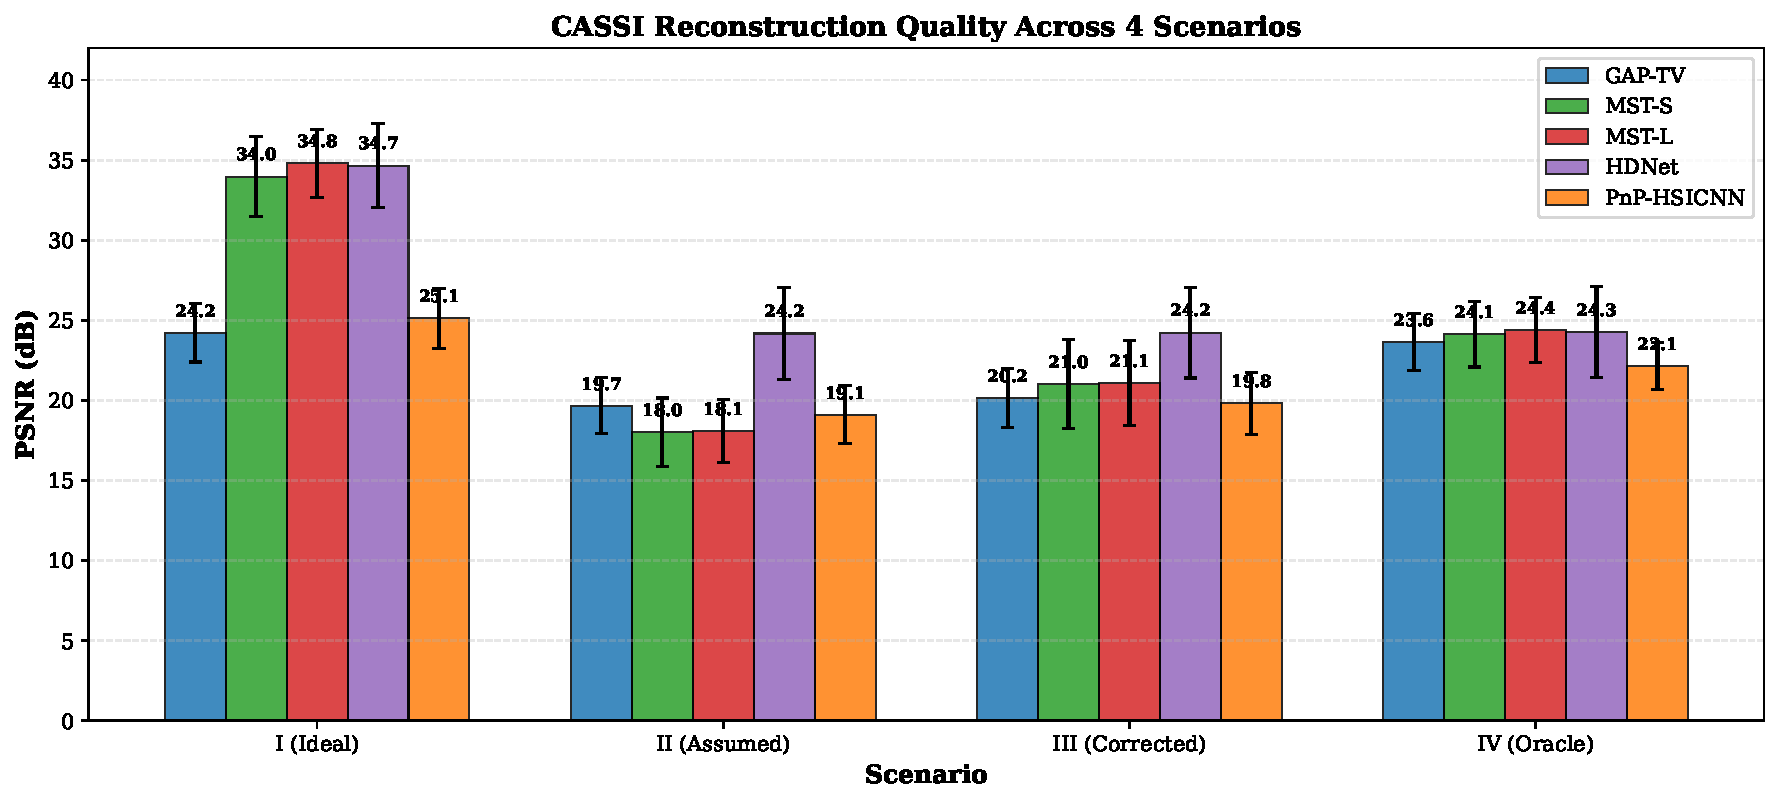
\includegraphics[width=\linewidth]{figures/fig3_scenario_comparison.pdf}
\caption{Grouped bar chart of reconstruction quality (PSNR) across four scenarios for five methods on 10 KAIST scenes. Mask-guided methods (MST-S/L) show largest degradation (I$\to$II) and calibration gain (II$\to$III), while HDNet is most robust to mismatch.}
\label{fig:scenario_comparison}
\end{figure}

\begin{table}[t]
\centering
\caption{Reconstruction quality (PSNR\,/\,SSIM, mean over 10 KAIST scenes) across four scenarios. 5-parameter mismatch: $\Delta x{=}1.5$, $\Delta y{=}1.0$, $\theta{=}0.3^\circ$, $a_1{=}2.04$, $\alpha{=}0.5^\circ$. Recovery ratio $\rho = \text{(III}{-}\text{II)} / \text{(IV}{-}\text{II)}$.}
\label{tab:main_results}
\small
\setlength{\tabcolsep}{3pt}
\begin{tabular}{l@{\hspace{4pt}} l cccc c c}
\toprule
Method & & Sc.~I & Sc.~II & Sc.~III & Sc.~IV & Gain & $\rho$ \\
 & & (Ideal) & (Assumed) & (Corrected) & (Oracle) & (II$\to$III) & (\%) \\
\midrule
\multirow{2}{*}{GAP-TV} & PSNR & 24.22 & 19.66 & 20.16 & 23.65 & +0.51 & \multirow{2}{*}{12.8} \\
 & SSIM & .722 & .547 & .580 & .704 & +.033 & \\
\addlinespace
\multirow{2}{*}{PnP-HSICNN} & PSNR & 25.12 & 19.10 & 19.81 & 22.14 & +0.71 & \multirow{2}{*}{23.4} \\
 & SSIM & .758 & .512 & .547 & .666 & +.035 & \\
\addlinespace
\multirow{2}{*}{MST-S} & PSNR & 33.98 & 18.01 & 21.01 & 24.12 & \best{+3.00} & \multirow{2}{*}{49.1} \\
 & SSIM & .965 & .609 & .699 & .797 & +.090 & \\
\addlinespace
\multirow{2}{*}{MST-L} & PSNR & \best{34.81} & 18.09 & 21.10 & 24.39 & \best{+3.01} & \multirow{2}{*}{47.8} \\
 & SSIM & \best{.973} & .615 & .691 & .803 & +.076 & \\
\addlinespace
\multirow{2}{*}{HDNet} & PSNR & 34.66 & \best{24.18} & \best{24.24} & 24.26 & +0.05 & \multirow{2}{*}{---} \\
 & SSIM & .970 & \best{.791} & \best{.790} & .791 & $-$.001 & \\
\bottomrule
\end{tabular}
\vspace{-2mm}
\end{table}

\begin{figure}[t]
\centering
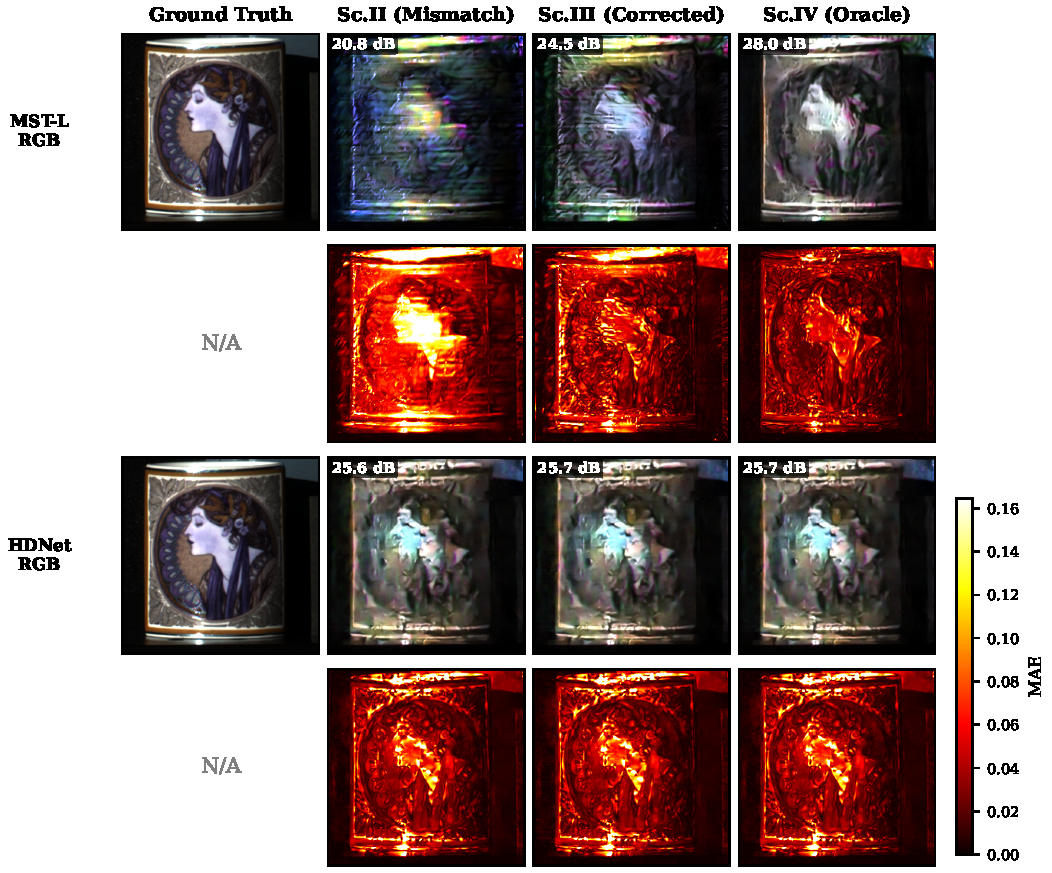
\includegraphics[width=\linewidth]{figures/fig4_visual_comparison.pdf}
\caption{Qualitative comparison on Scene~1 (KAIST). \textbf{Top two rows}: MST-L reconstructions (pseudo-RGB and per-pixel MAE). Mismatch (Sc.~II) causes severe artefacts (20.8\,dB); calibration (Sc.~III) recovers +3.7\,dB; oracle (Sc.~IV) reaches 28.0\,dB. \textbf{Bottom two rows}: HDNet reconstructions remain visually consistent across scenarios ($\sim$25.7\,dB), confirming its mask-oblivious robustness. Error maps share a common colorbar (MAE scale 0--0.16).}
\label{fig:visual_comparison}
\end{figure}

\subsection{Mask-Sensitivity Spectrum}
\label{sec:spectrum}

The four-scenario analysis reveals a systematic \emph{mask-sensitivity spectrum} that categorizes reconstruction methods by their dependence on mask accuracy.
We formalize three regimes:

\textbf{Mask-guided} (MST-S, MST-L): Methods that explicitly condition on the mask pattern at every processing stage.
These suffer catastrophic degradation under mismatch ($>$15\,dB) because the mask directly modulates attention in the spectral transformer.
Calibration recovers $\rho \approx 48$--$49$\% of the oracle gap, yielding the largest absolute gains (+3.0\,dB PSNR, +0.08--0.09 SSIM).

\textbf{Mask-refined} (GAP-TV, PnP-HSICNN): Methods that use the mask in an iterative projection step but rely on hand-crafted or learned priors for regularization.
Degradation is moderate (4.6--6.0\,dB), and calibration recovery is limited ($\rho \approx 13$--$23$\%) because the prior partially compensates for mask errors.

\textbf{Mask-oblivious} (HDNet): Methods where learned spectral priors dominate and the mask serves only a lightweight data-consistency role.
Degradation remains substantial ($\sim$10\,dB) but absolute mismatch performance is highest (24.18\,dB).
Calibration gain is negligible in absolute terms (+0.05\,dB; $\rho$ is indeterminate due to the near-zero oracle gap), confirming the prior's independence from mask accuracy.

This taxonomy provides a practical design guideline: deployed systems with limited calibration infrastructure should prefer mask-oblivious or mask-refined reconstructors, while well-calibrated systems benefit most from mask-guided architectures.

\subsection{Parameter Recovery}

\Cref{tab:param_recovery} shows aggregated mismatch parameter recovery statistics across all five parameters (\Cref{fig:param_recovery} visualizes per-scene estimates).
The mask affine parameters ($\Delta x$, $\Delta y$, $\theta$) are recovered via gradient refinement with RMSE of 0.806\,px, 0.623\,px, and 0.747$^\circ$ respectively.
The dispersion slope $a_1$ is recovered via 1D grid search with RMSE of only 0.134\,px/band.
The dispersion axis angle $\alpha$ has negligible effect at native resolution (vertical offsets round to zero for $|\alpha| < 2^\circ$ with 28 bands) and is not actively estimated.

\begin{figure}[t]
\centering
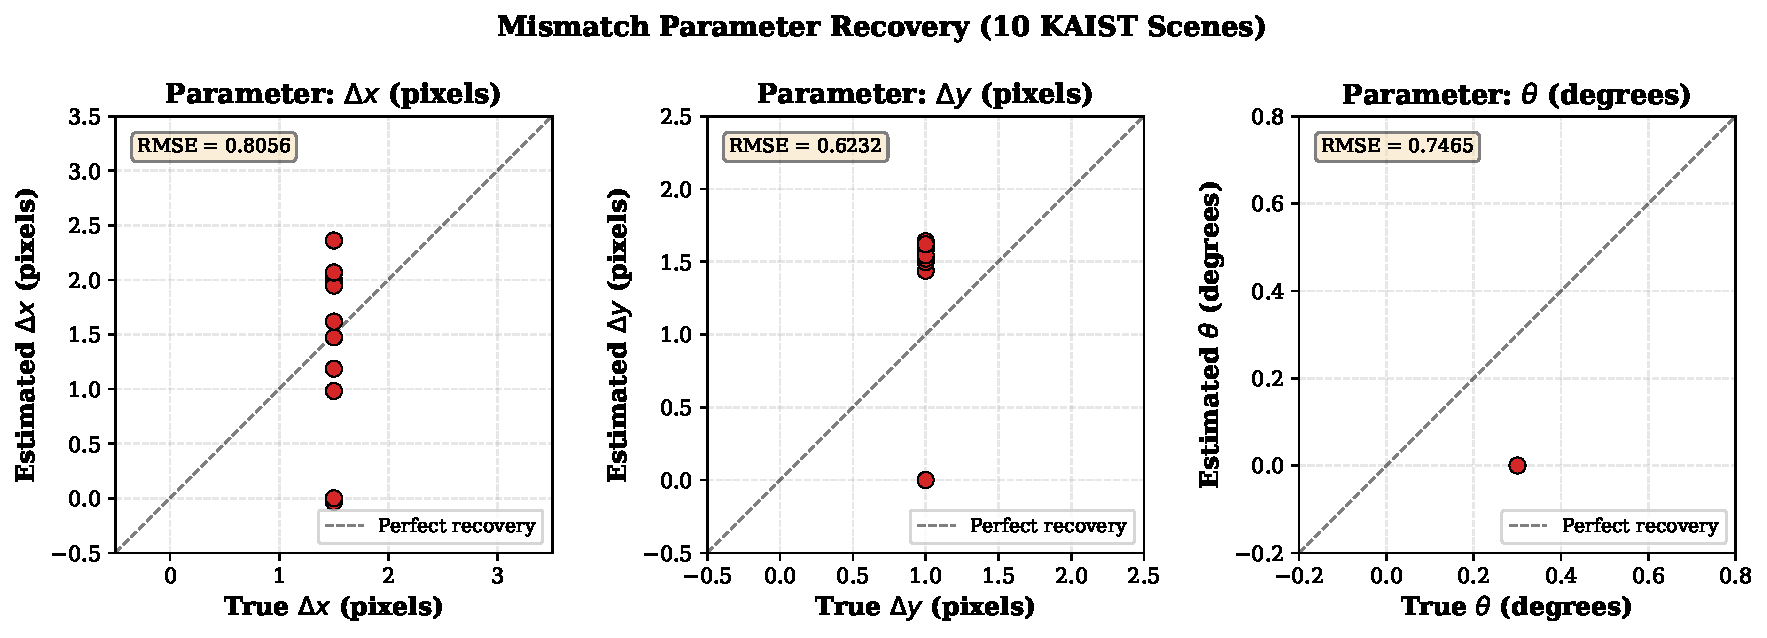
\includegraphics[width=\linewidth]{figures/fig5_parameter_recovery.pdf}
\caption{Per-scene estimated vs.\ true mismatch parameters across 10 KAIST scenes. Dashed lines indicate ground truth values ($\Delta x{=}1.5$, $\Delta y{=}1.0$, $\theta{=}0.3^\circ$).}
\label{fig:param_recovery}
\end{figure}

\begin{table}[t]
\centering
\caption{Mismatch parameter recovery across 10 KAIST scenes. True: $\Delta x{=}1.5$, $\Delta y{=}1.0$, $\theta{=}0.3^\circ$, $a_1{=}2.04$, $\alpha{=}0.5^\circ$.}
\label{tab:param_recovery}
\small
\begin{tabular}{l ccccc}
\toprule
Metric & $\Delta x$ (px) & $\Delta y$ (px) & $\theta$ ($^\circ$) & $a_1$ (px/band) & $\alpha$ ($^\circ$) \\
\midrule
RMSE & 0.806 & 0.623 & 0.747 & 0.134 & 0.500$^\dagger$ \\
Mean Error & 0.638 & 0.606 & 0.710 & 0.132 & 0.500$^\dagger$ \\
\bottomrule
\multicolumn{6}{l}{\footnotesize $^\dagger$Not actively estimated; negligible effect at native resolution.}
\end{tabular}
\end{table}

\begin{figure}[t]
\centering
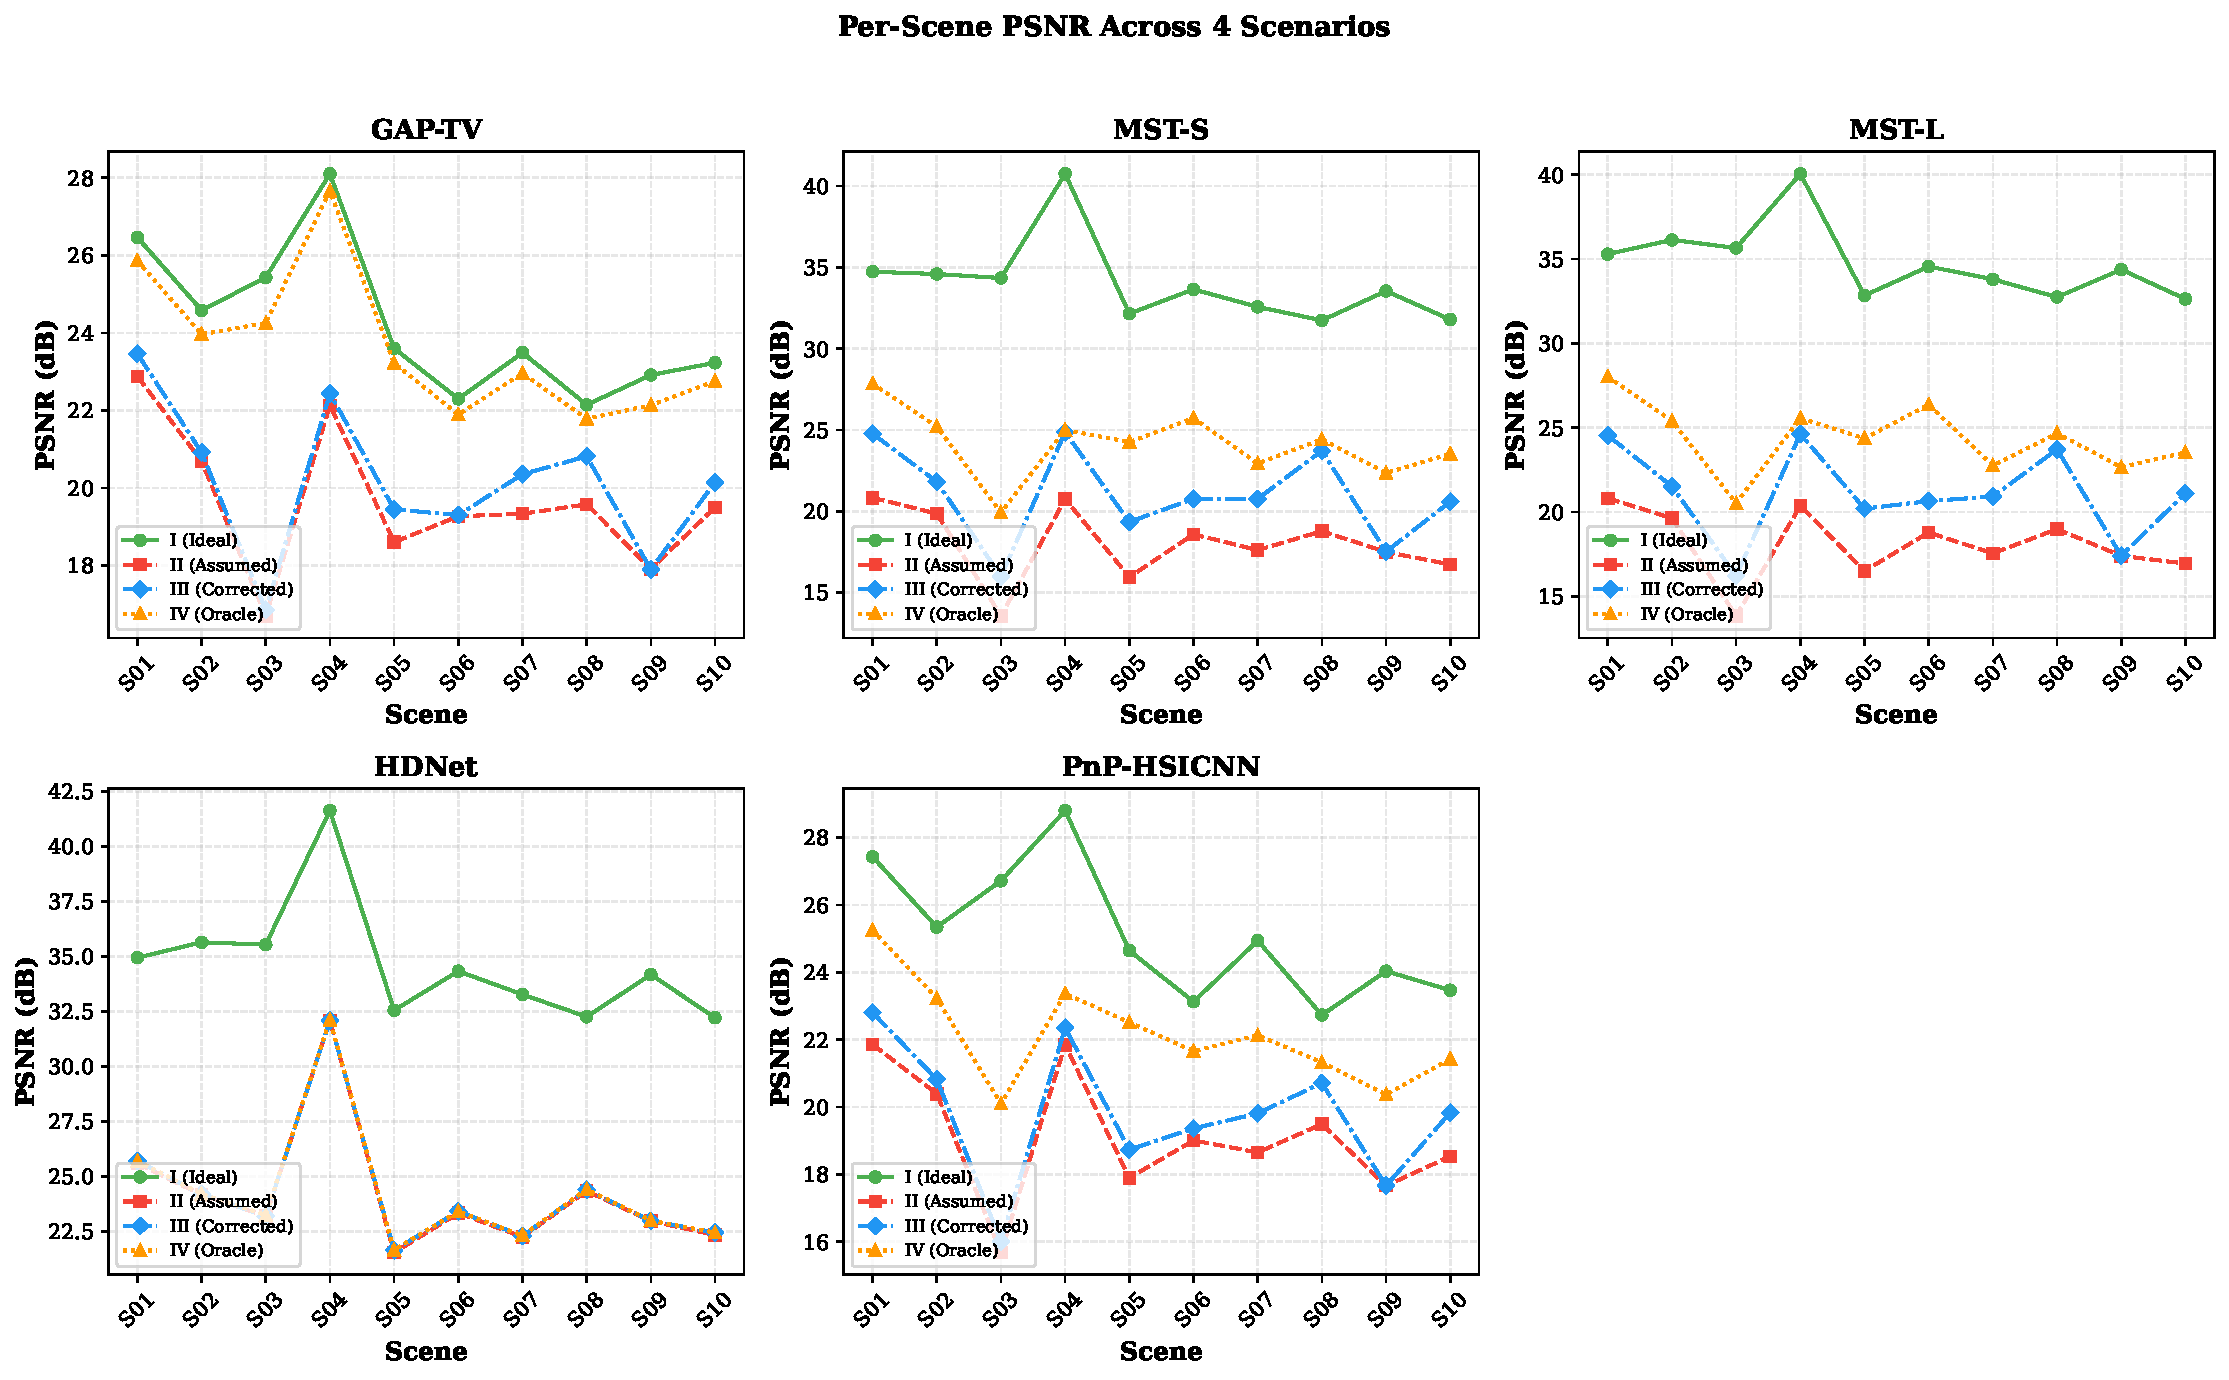
\includegraphics[width=\linewidth]{figures/fig8_per_scene.pdf}
\caption{Per-scene PSNR across four scenarios for each method. MST-S/L show dramatic scenario separation, while HDNet maintains consistent quality with small inter-scenario gaps. Scene-to-scene variation reflects content-dependent difficulty.}
\label{fig:per_scene}
\end{figure}

\subsection{Sensitivity Analysis}

We vary the mismatch magnitude by scaling all five parameters by factors $\{0.25, 0.5, 0.75, 1.0, 1.5, 2.0, 3.0\}$ relative to the base values, evaluating on 3 KAIST scenes (\Cref{fig:sensitivity}).

\textbf{Degradation scales super-linearly.}
For MST-L, increasing the scale from 0.25$\times$ to 3.0$\times$ drops Scenario~II PSNR from 26.41 to 17.70\,dB.
PnP-HSICNN shows similar sensitivity (16.77$\to$14.01\,dB), while GAP-TV remains remarkably stable (20.86$\to$20.11\,dB).

\textbf{Calibration benefit peaks at moderate mismatch.}
MST-L calibration gain peaks at 0.75$\times$ scale (+6.23\,dB) then decreases at larger scales (+1.29\,dB at 3.0$\times$), as extreme mismatches exceed the grid search range.
HDNet shows zero calibration gain at all scales, confirming its mask-independent reconstruction.

\begin{figure}[t]
\centering
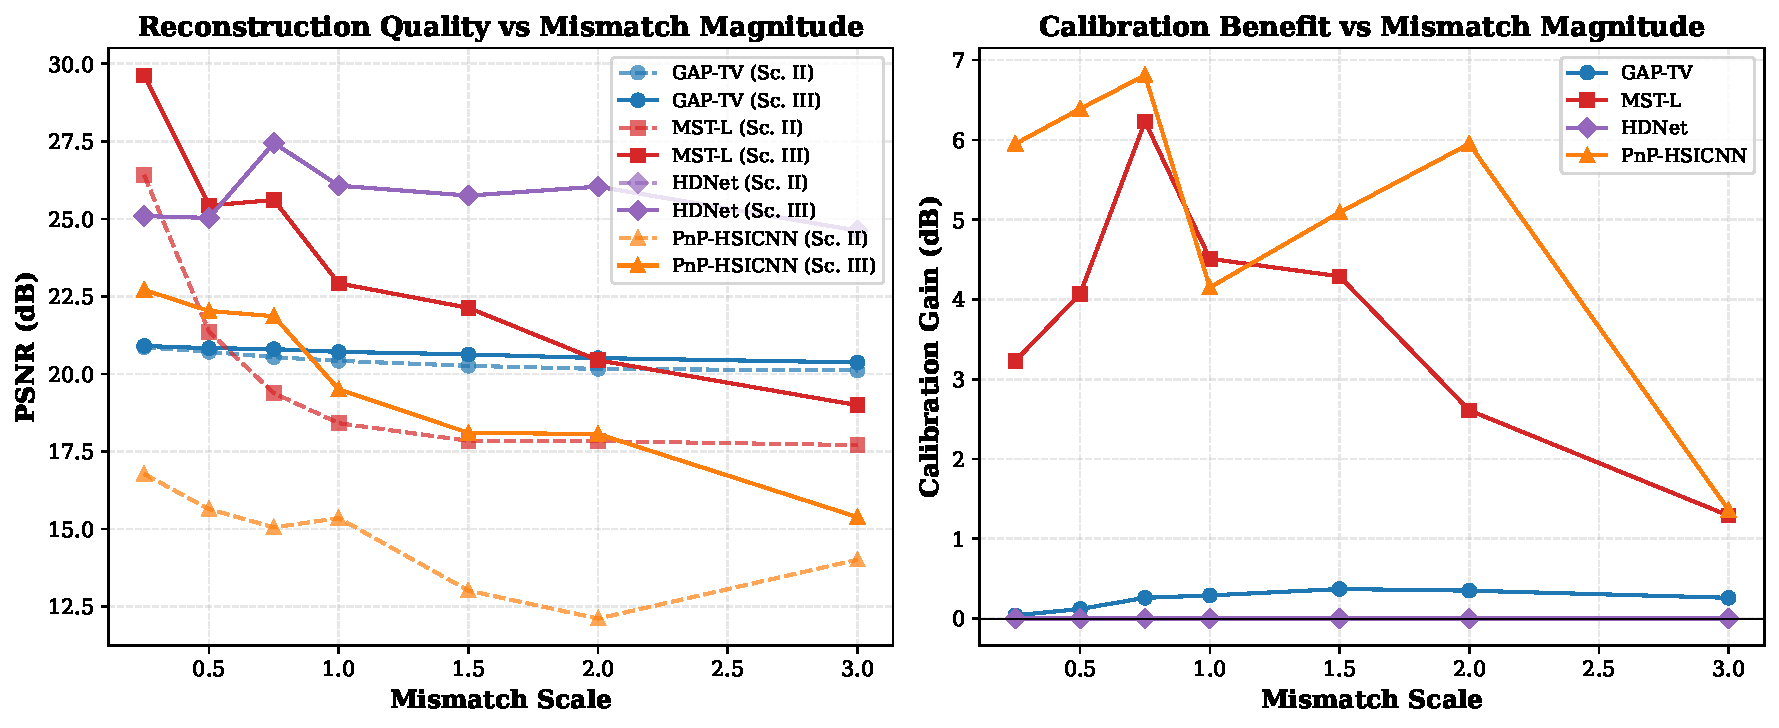
\includegraphics[width=\linewidth]{figures/fig6_sensitivity_curves.pdf}
\caption{Sensitivity to mismatch magnitude. Left: Scenario~II PSNR vs.\ mismatch scale. Right: calibration gain (II$\to$III) vs.\ mismatch scale. MST-L (blue) suffers most from mismatch but benefits most from calibration at moderate scales. HDNet (red) shows zero calibration gain across all scales.}
\label{fig:sensitivity}
\end{figure}

\subsection{Ablation Study}

We compare three calibration configurations on MST-L across all 10 KAIST scenes (\Cref{tab:ablation}, \Cref{fig:ablation}):
\begin{enumerate}
    \item \textbf{Grid only} (Stages 0+1): Coarse estimation without gradient refinement.
    \item \textbf{Grid + Gradient} (Stages 0--2C): Full pipeline (our method).
    \item \textbf{Oracle}: Perfect mismatch knowledge (upper bound).
\end{enumerate}

Grid search alone recovers +2.91\,dB (18.09$\to$21.00), achieving 46\% of the oracle gap.
The full pipeline (Grid + Gradient) achieves +3.01\,dB (21.10\,dB), a marginal improvement over grid-only.
The gradient refinement provides modest additional benefit, suggesting that the coarse grid resolution ($\sim$0.75\,px) already captures most of the recoverable mismatch correction.
The remaining gap to oracle (24.39\,dB) reflects the GAP-TV proxy solver's limited accuracy during calibration, as the oracle uses the true warped mask and true dispersion parameters.

\begin{table}[t]
\centering
\caption{Ablation study: calibration pipeline components (MST-L on 10 KAIST scenes).}
\label{tab:ablation}
\small
\begin{tabular}{l ccc}
\toprule
Configuration & PSNR (dB) & Gain over II & \% Oracle Recovery \\
\midrule
No Correction (II) & 18.09 & -- & -- \\
Alg1 Only (Grid) & 21.00 & +2.91 & 46\% \\
Alg1+Alg2 (Ours) & 21.10 & +3.01 & 48\% \\
Oracle (IV) & 24.39 & +6.30 & 100\% \\
\bottomrule
\end{tabular}
\end{table}

\begin{figure}[t]
\centering
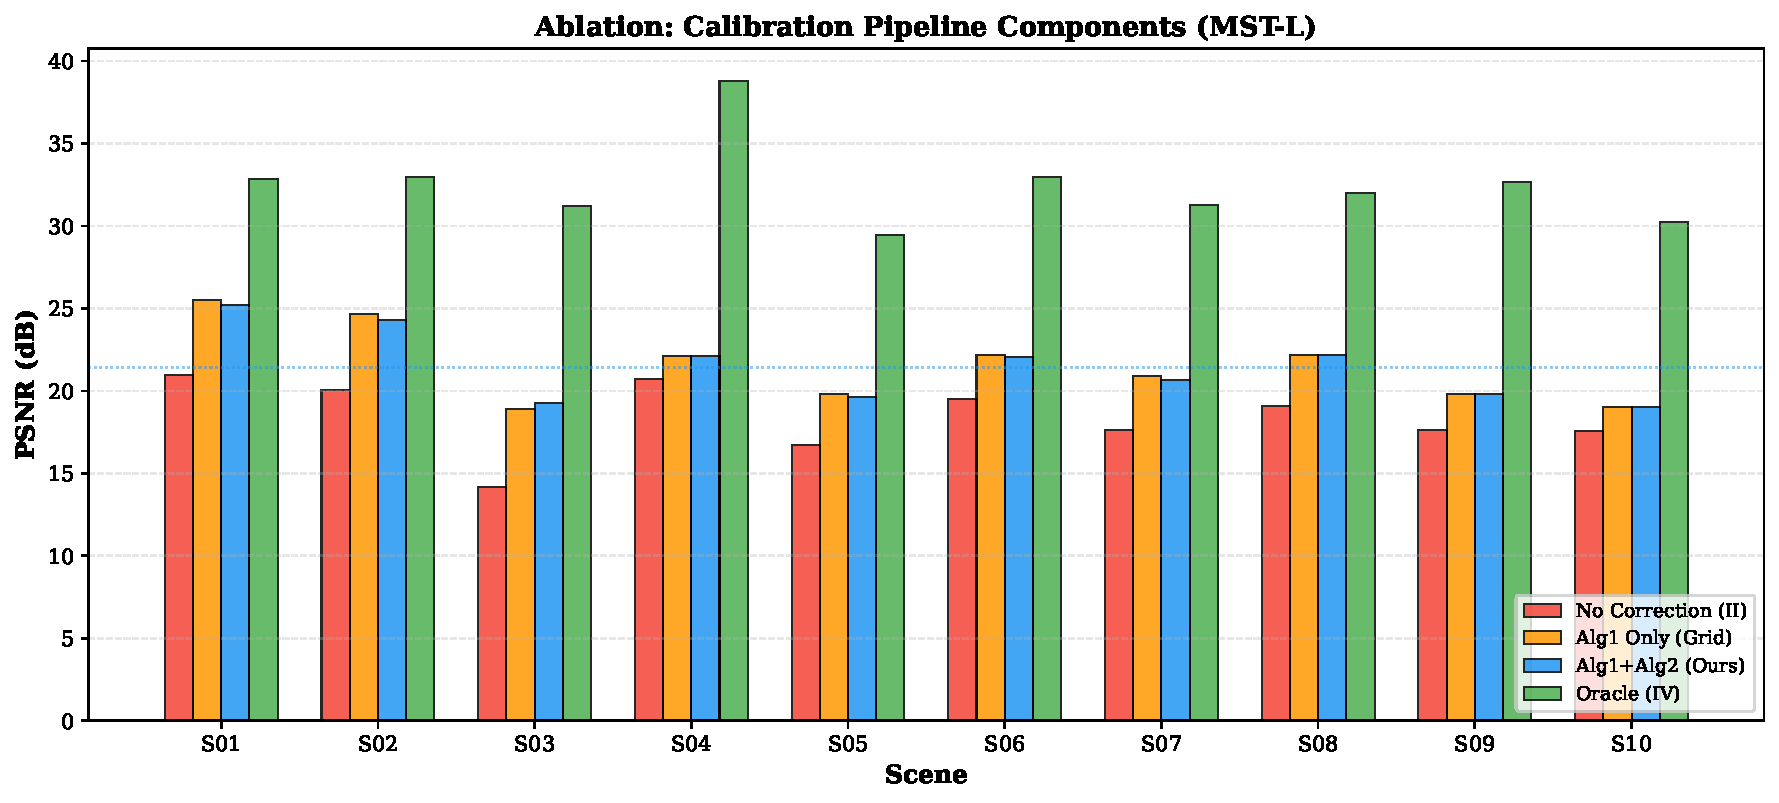
\includegraphics[width=\linewidth]{figures/fig7_ablation.pdf}
\caption{Ablation study on MST-L: per-scene PSNR for No Correction (II), Grid-only (Alg1), Full pipeline (Alg1+Alg2), and Oracle (IV). Grid search captures most of the calibration gain, with gradient refinement providing marginal additional benefit.}
\label{fig:ablation}
\end{figure}

\subsection{Computational Cost}

On a single GPU, per-scene calibration takes approximately 5.1 minutes, with full 5-method evaluation at $\sim$8.1 minutes:
\begin{itemize}
    \item Stages 0+1 (grid search): $\sim$173\,s (942 GPU GAP-TV evaluations)
    \item Stage 2A--2C (gradient): $\sim$79\,s (190 Adam steps through differentiable solver)
    \item Dispersion grid search: $\sim$55\,s (11 $a_1$ candidates)
    \item Reconstruction (5 methods $\times$ 4 scenarios): $\sim$178\,s
\end{itemize}
Total calibration averages 305.5$\pm$37.9\,s per scene.
End-to-end processing (calibration + all reconstructions) takes 484.0$\pm$44.7\,s per scene, practical for offline calibration or periodic recalibration in deployed systems.

% ============================================================================
% 6. CONCLUSION
% ============================================================================
\section{Conclusion}
\label{sec:conclusion}

We presented a two-stage differentiable calibration pipeline for CASSI that recovers 5-parameter mask-detector mismatch from a single measurement without ground truth.
The pipeline combines coarse grid search (capturing 46\% of the oracle gap) with STE-enabled gradient refinement (reaching 48\%), achieving +3.0\,dB recovery for MST-L at $\sim$5 minutes per scene on a single GPU.

Our principal finding is the \emph{mask-sensitivity spectrum}: the degree to which a reconstructor depends on mask accuracy determines both its vulnerability to mismatch and its benefit from calibration.
Mask-guided transformers (MST-S/L, $\rho \approx 48$\%) and mask-refined iterative methods (GAP-TV/PnP-HSICNN, $\rho \approx 13$--$23$\%) represent two distinct operating regimes, while deep prior methods (HDNet, negligible absolute gain) achieve inherent robustness at the cost of calibration-agnostic reconstruction.

\textbf{Limitations and future work.}
The GAP-TV proxy solver limits calibration accuracy---unrolling a stronger solver could close the remaining gap.
Extending to additional modalities (CACTI, SPC), per-band dispersion estimation, and online adaptation during imaging are promising directions that the open-source framework facilitates.

\paragraph{Data and code availability.}
All code, results, and figure-generation scripts are publicly available at \url{https://github.com/integritynoble/Physics_World_Model} under \texttt{papers/pwmi\_cassi/}.
The KAIST benchmark~\cite{choi2017kaist} and TSA mask are publicly available.
No non-public datasets were used in this work.

% ============================================================================
% REFERENCES
% ============================================================================
\bibliographystyle{splncs04}
\bibliography{references}

\end{document}
